\documentclass[12pt]{article}
\usepackage[utf8]{inputenc}
\usepackage[T1]{fontenc}
\usepackage{titlesec}
\usepackage[inline]{enumitem}
\usepackage[left=2.54cm,top=3cm,right=2.54cm,bottom=3cm]{geometry}
\usepackage[sorting=none, style=numeric-comp]{biblatex}
\usepackage{hyperref}
\usepackage{graphicx}
% \usepackage{upgreek}
% \usepackage{setspace}
% \usepackage{longtable}
\usepackage{tabularx}
% \usepackage{framed}
% \usepackage{eurosym}
\usepackage{listings}
% \usepackage{rotating}
% \usepackage[table]{xcolor}
\usepackage[acronym,toc,nogroupskip,nopostdot]{glossaries}
\usepackage{glossary-mcols}
\usepackage[justification=centering]{caption}
\usepackage{pdfpages}

% \graphicspath{ {00images/} }
\DeclareGraphicsExtensions{.png,.pdf,.jpg}
% \DeclareGraphicsExtensions{.pdf,.png} % - CHANGE TO THIS

\addbibresource{mendeley.bib}
\setlength{\parindent}{1cm}

%\onehalfspacing
% Acronyms %%%%%%%%
\makeglossaries

\newacronym{bmc}{BMC}{Business Model Canvas}
\newacronym{ml}{ML}{Machine learning}
\newacronym{sla}{SLA}{Service Level Agreement}
\newacronym{ms}{MS}{Microsoft}
\newacronym{hw}{HW}{hardware}
\newacronym{sw}{SW}{software}
%\newacronym{}{}{}
%\newacronym{}{}{}

\makeglossaries

%%%%%%%%%%%%%%%%%%% 

\begin{document}

% \includepdf{frontpage}

\tableofcontents
% \pagebreak

% \begin{singlespacing}
% \setglossarystyle{mcolindex}
% \printglossary[type=\acronymtype, title=List of acronyms and abbreviations, toctitle=List of acronyms and abbreviations, nonumberlist]
% \printglossary
% \end{singlespacing}

\pagebreak

\section{Introduction}

In the days of great technical advance, in which we are right now, everybody would like to have the service they offer to be the fastest, the best and the most intelligent, so that they can beat the competition. To keep up with a technological advance at such a fast pace, many companies are choosing to base their services on cloud as it is relatively inexpensive compared to buy dedicated hardware each time. Scalability, accessibility, mobility and redundancy are other advantages. Therefore, many big players such as Google, Microsoft or Amazon are offering cloud based services to enterprises.

Knowing what might be a business model of these giants and what obstacles they might be facing is interesting. Therefore, this synopsis will look into the Economy of Cloud-bases Machine Learning services offered by Microsoft and theories learned at Entrepreneurship, Innovation and Business models will be applied, in particular Business model Canvas, Network effect, Path dependency and Lock-in and Transaction costs.

% 
% \begin{figure}[ht]
%     \centering
%     \includegraphics[width=0.8\textwidth]{00images/arch-ver1}
%     \caption{Simplest version of the architecture. Each sensor communicates directly with the collection point.}
%     \label{fig:arch-ver1}
% \end{figure}
\section{Problem formulation}
\section{Theories}

% TODO write intro to the theories chapter

\subsection{Business Model}\label{sec:business-model}

There are various different definitions of a business model. Arguably the most popular one is as follows: \textit{``business model describes the rationale of how an organisation creates, delivers, and captures value}''~\cite{Osterwalder2010BusinessChallengers}. The business model is an important tool to conceptualise and record the relations and environment within which the organisation operates. Two approaches to business models are particularly interesting:
\begin{enumerate*}[label=(\roman*)] 
    \item The STOF model by Bouwmann et. al., which focuses on providing value for both customers and businesses by balancing the customers' requirements and strategic business interests~\cite{Bouwman2008ServiceModels}; and the
    \item \acrfull{bmc} by Osterwalder et. al. which puts more focus on simplicity and plug\&play approach for idea sharing and mapping~\cite{Hong2013CriticismsCanvas}.
\end{enumerate*}
 
In this synopsis, we further focus on the second one. Its main goal is to provide entrepreneurs, businessmen, investors and other people with a common language for discussing business model and innovation of a specific organisation. The canvas consists of 9 building blocks that are divided into four areas of an organisation: customers, offer, infrastructure and financial viability.

In the original definition of \acrshort{bmc}, the basic goal of an organisation is to make money~\cite[p. 21]{Osterwalder2010BusinessChallengers} and thus this canvas cannot be used by other types of organisations (e.g. NGOs, social enterprises). Although this has been criticised in the literature~\cite{Hong2013CriticismsCanvas}, we believe this does not prevent the \acrshort{bmc} to be widely adopted, nor does it prevent it to be applied on our scenario.

Further criticism of the \acrshort{bmc} include lack of consideration for competition or imbalance in the focus on different building blocks~\cite{Hong2013CriticismsCanvas}.

% TODO write about BMC applied to Azure/Microsoft/AI computing
\paragraph{Application of BMC to cloud-based machine learning services}
To better understand how the machine learning services can be provided as a cloud-based solution, we created a \acrshort{bmc}. We used a modified version of the original canvas called \textit{Advanced Business Model Canvas}, which adds sub-points into some of the boxes, making it easier to avoid ambiguity when filling the \acrshort{bmc}~\cite{King2017BusinessInstructions, Hong2013CriticismsCanvas}. The \acrshort{bmc} can be found in Appendix 1.
% TODO add reference to appendix

After filling the canvas using Microsoft's Azure Machine Learning Studio\footnotemark as an example of a service, we find that the business model used by Microsoft is sound and usable in the market. To our best knowledge, Microsoft does not currently offer consultancy services for the design of the \acrshort{ml} solution.
% 
\footnotetext{\url{https://studio.azureml.net/}, accessed 09-12-2018}
% 
Limited advice on how to achieve the best results, using Microsoft's solution is published with the documentation\footnotemark and best practice techniques can also be found in various online communities. The support provided by Microsoft, however is limited to how to use different parts of the tool and error handling. Large enterprise customers may also engage in \acrshort{sla} specifications. We find that the consultancy offering might further complement Microsoft's Machine Learning environment and bring additional source of revenue to the company.
% 
\footnotetext{\url{https://docs.microsoft.com/en-us/azure/machine-learning/studio/faq}, accessed 09-12-2018}

Based on this case, we also maintain that the sub-points are not an obstacle to the original purpose of the \acrshort{bmc}, as they do help with filling the canvas with relevant information. 
\section{Conclusion}\label{sec:conclusion}

In this Synopsis, four economic theories taught this semester were applied: Business model Canvas, Network effect, Path dependency and Lock-in and Transaction costs.

The \textit{Business Model Canvas} has been filled and all blocks identified to analyse how a big player, such as Microsoft, may be generating revenue and approaching the potential customers. Thanks to this knowledge, the effect of \textit{Network economics} could be explored, identifying the incompatibility of services of biggest players as their biggest weaknesses and strengths. It is also important to know what are the areas, in which the decision made in past, can have a negative impact in the future in order to avoid such decisions and therefore, \textit{Path dependency and Lock-in} theories have been investigated. The last theory looked into was \textit{Transaction cost}, where the Microsoft's current inability to manufacture needed equipment in-house for purposes of his cloud, was identified as one of the biggest transaction costs.

As the technology matures further and the use cases become more clear, we can expect more competition in the field and perhaps even offering of a cloud-based \acrshort{ml} service as a standalone system (as opposed to a bundle offering, tied with other cloud services). It is challenging to objectively evaluate the economic performance of the cloud-based \acrshort{ml} system, as this is currently always bundled with other cloud-based services.
% 
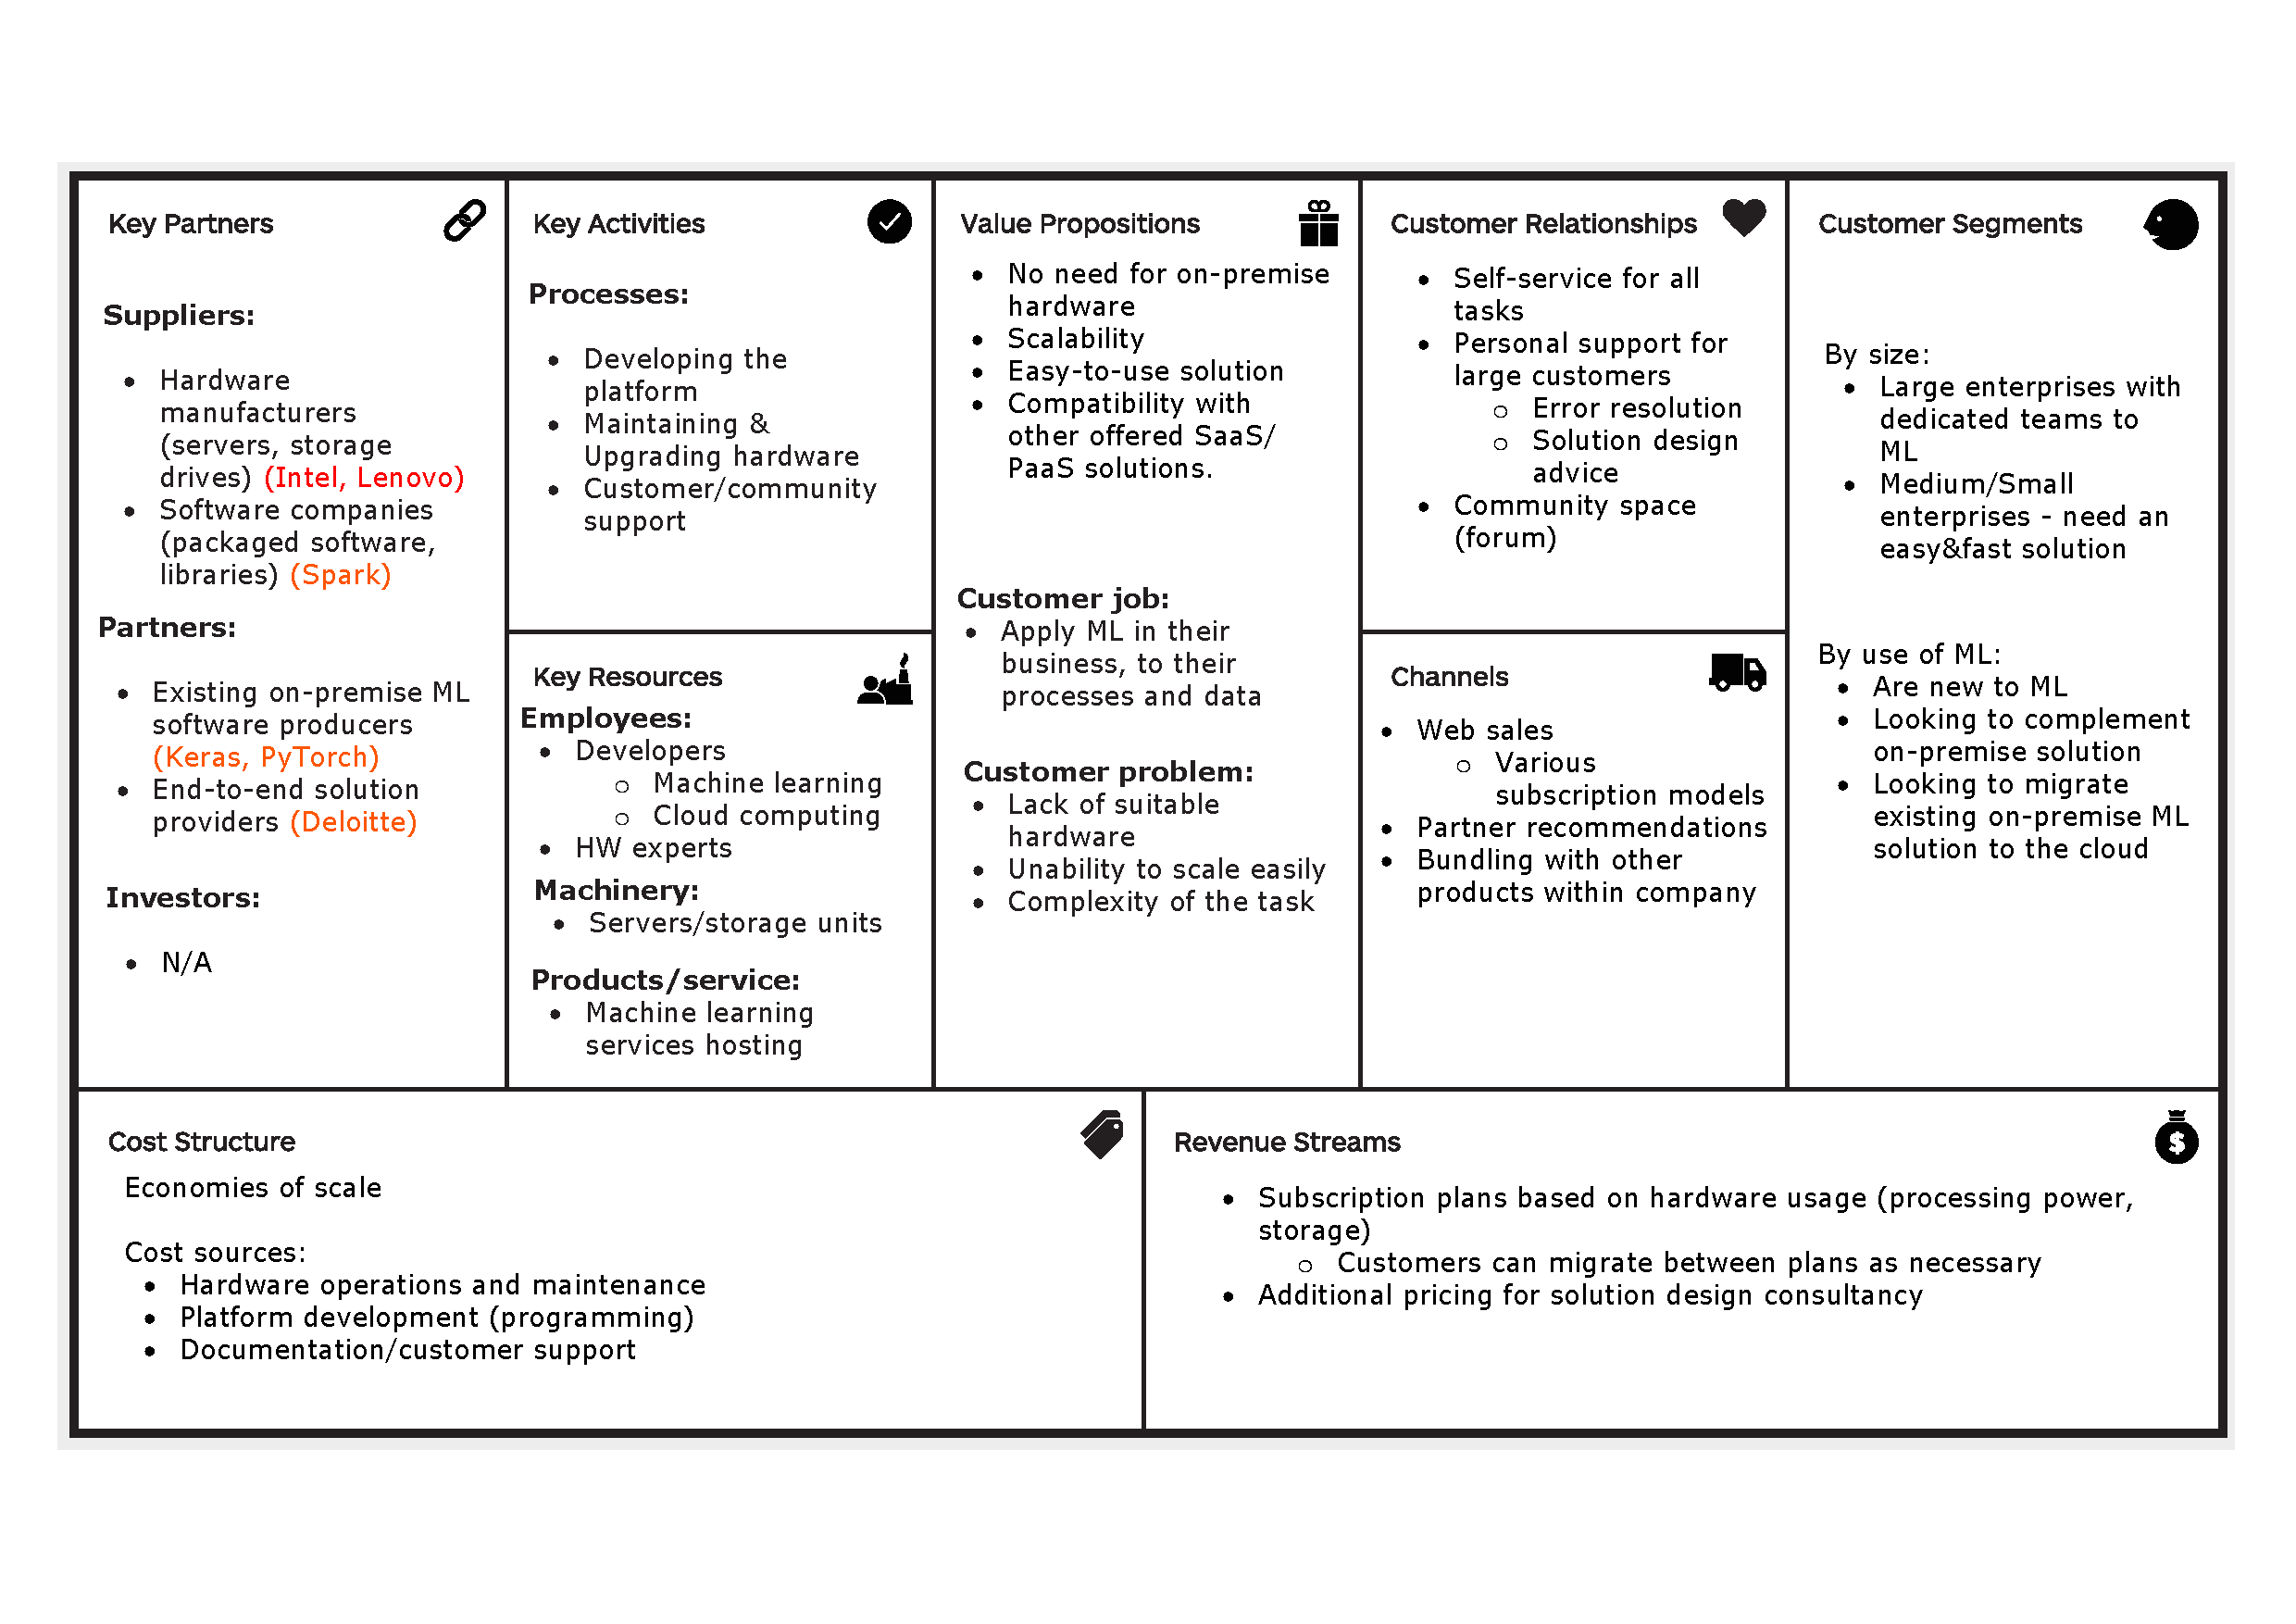
\includepdf[angle=90]{bmc.pdf}
% 

\printbibliography[heading=bibintoc]
\pagebreak

\end{document}